% Short class talk (5-6 minutes). Build: make (slides PDF and speaker-notes PDF).
\documentclass[aspectratio=169,10pt]{beamer}
% shared preamble for the final presentation and the class talk
\usetheme[progressbar=frametitle,numbering=fraction]{metropolis}
\usepackage[T1]{fontenc}
\usepackage[default]{lato}
\usepackage[scaled=0.85]{DejaVuSansMono}
\usepackage{booktabs,tabularx,array,xcolor,tikz,pgfpages,listings}
\usetikzlibrary{arrows.meta,positioning,fit,calc,shapes.geometric}
\definecolor{ink}{HTML}{17262B}\definecolor{acc}{HTML}{1F5FAD}\definecolor{ok}{HTML}{2E7D32}
\definecolor{warn}{HTML}{D9822B}\definecolor{pale}{HTML}{EEF3F8}
\setbeamercolor{frametitle}{bg=ink}
\setbeamercolor{progress bar}{fg=acc}
\setbeamercolor{alerted text}{fg=acc}
\setbeamertemplate{note page}[plain]
\usepackage{xspace}
\newcommand{\pg}{PostgreSQL\xspace}
\newcolumntype{L}[1]{>{\raggedright\arraybackslash}p{#1}}
\newcolumntype{Y}{>{\raggedright\arraybackslash}X}
\newcommand{\ok}[1]{\textcolor{ok}{\textbf{#1}}}
\newcommand{\wa}[1]{\textcolor{warn}{\textbf{#1}}}
\tikzset{
  box/.style={draw=acc,rounded corners=2pt,align=center,fill=pale,font=\scriptsize,minimum height=9mm,text width=22mm},
  io/.style={draw=gray,align=center,fill=gray!10,font=\scriptsize,minimum height=8mm,text width=19mm},
  orc/.style={draw=ok,rounded corners=2pt,align=center,fill=ok!8,font=\scriptsize,minimum height=7mm,text width=22mm},
  fl/.style={-{Stealth[length=1.6mm]},thick,draw=ink},
  bk/.style={-{Stealth[length=1.6mm]},dashed,draw=acc}}

\ifdefined\shownotes\setbeameroption{show only notes}\fi
\title{Grammar-Aware Fuzzing of PostgreSQL, and Beyond}
\subtitle{CS-5187 Software Analysis, Term Project A3}
\author{Venu Kummari \and Bhuvan Chilukuti \and Gowtham Reddy}
\institute{IIT Guwahati}
\date{November 2026}

\begin{document}

\maketitle
\note{VENU (15 s). Good afternoon. We built a fuzzer, a dynamic-analysis tool that writes test
queries for PostgreSQL and decides by itself when an answer is wrong. Then we generalized it to
four more SQL engines. Nine PostgreSQL bugs reported, seven fixed upstream, five with our patches;
three more fixes filed to DuckDB, Turso and DataFusion.}

\begin{frame}{Target and problem}
\begin{columns}[T]
\column{0.52\textwidth}
\begin{itemize}
  \item \textbf{Target}: \pg master built with \textbf{assertions}; reference: release 18.6.
  \item \textbf{Bug classes}: crash/assertion, \alert{wrong result}, internal error, hang.
  \item A wrong result leaves no error and no log line: the tool needs a \alert{test oracle} that knows the right answer.
\end{itemize}
\column{0.44\textwidth}
\begin{block}{Our idea}
Generate SQL as \alert{typed derivation trees}. Rewrite each tree into
\alert{equivalent queries}, run it under \alert{other plans} and on the
\alert{last release}. Any disagreement is a bug.
\end{block}
\end{columns}
\end{frame}
\note{VENU (30 s). PostgreSQL is one of the most used databases and its planner changes every
week. The worst bugs return wrong rows silently. A fuzzer can run millions of queries; the hard
part, the oracle problem, is to know when an answer is wrong. We decide by comparison: equivalent
questions must give equal answers.}

\begin{frame}{Arbor: architecture and techniques}
\centering\resizebox{0.9\linewidth}{!}{% architecture of the PostgreSQL fuzzer
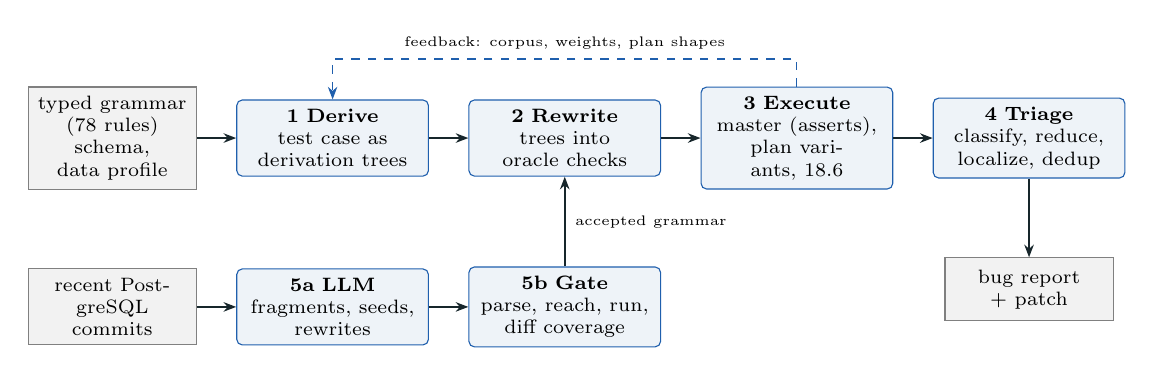
\begin{tikzpicture}[node distance=4mm and 5mm]
\node[io] (g) {typed grammar (78 rules)\\schema, data profile};
\node[box,right=of g] (s1) {\textbf{1 Derive}\\test case as\\derivation trees};
\node[box,right=of s1] (s2) {\textbf{2 Rewrite}\\trees into\\oracle checks};
\node[box,right=of s2] (s3) {\textbf{3 Execute}\\master (asserts),\\plan variants, 18.6};
\node[box,right=of s3] (s4) {\textbf{4 Triage}\\classify, reduce,\\localize, dedup};
\node[io,below=10mm of g] (c) {recent \pg commits};
\node[box,right=of c] (l1) {\textbf{5a LLM}\\fragments, seeds,\\rewrites};
\node[box,right=of l1] (l2) {\textbf{5b Gate}\\parse, reach, run,\\diff coverage};
\node[io,below=10mm of s4] (r) {bug report\\+ patch};
\draw[fl] (g)--(s1); \draw[fl] (s1)--(s2); \draw[fl] (s2)--(s3); \draw[fl] (s3)--(s4); \draw[fl] (s4)--(r);
\draw[bk] (s3.north) -- ++(0,0.35) -| node[pos=0.25,above,font=\tiny]{feedback: corpus, weights, plan shapes} (s1.north);
\draw[fl] (c)--(l1); \draw[fl] (l1)--(l2); \draw[fl] (l2.north) -- node[right,font=\tiny]{accepted grammar} (s2.south -| l2.north);
\end{tikzpicture}
}
\scriptsize
\begin{columns}[T]
\column{0.5\textwidth}
\begin{itemize}
  \item \textbf{Typed grammar} (own DSL, 78 rules): 99.3\% valid statements (random mutation 26\%); tree kept for every query.
  \item \textbf{Oracles}: crash/assertion, internal error, hang; 18 \textbf{plan variants}; \textbf{metamorphic tree rewrites} (TLP, NoREC, $e\rightarrow(\mathrm{SELECT}\ e)$); \textbf{cross-version}; \textbf{CERT} estimates.
\end{itemize}
\column{0.5\textwidth}
\begin{itemize}
  \item \textbf{Triage}: reproduce $\times3$, reduce on the tree (smallest derivation of the same type), localize to a plan setting, rewrite or version.
  \item \textbf{LLM} reads recent commits and proposes grammar; a \textbf{gate} on the server accepts it only if it runs and executes the commit's changed lines.
\end{itemize}
\end{columns}
\end{frame}
\note{GOWTHAM (60 s). Five steps. One: derive a test case from our typed grammar; types make every
query valid, so the server spends its time planning, not rejecting syntax. Two: rewrite the tree
into checks; for example TLP splits a query into the rows where a condition is true, false and
NULL, and the parts must add up to the whole. Three: run on master, under other planner settings
and on release 18.6. Four: triage shrinks the failure on the tree and finds which setting or
rewrite flips it. Five: an LLM reads recent commits and proposes grammar, but PostgreSQL decides
what enters.}

\begin{frame}{Arbor: all nine bugs and how they were found}
\scriptsize
\begin{tabularx}{\linewidth}{@{}L{0.18\linewidth}L{0.24\linewidth}YL{0.17\linewidth}@{}}
\toprule
Bug type & Found by & Signal & Upstream \\
\midrule
assertion (crash) & LLM fragment + TLP check & assertion during a metamorphic check & \ok{fixed} \#19803 \\
wrong output & cross-version oracle & master and 18.6 disagreed & \ok{fixed, our patch} \#19771 \\
assertion (crash) & extended-statistics generator & assertion in the estimator & \ok{fixed, our patch} \\
wrong result + assertion & grammar fuzzer + cross-version & assertion on master, wrong answer on 18.6 & \ok{fixed, our patch} \#19768 \\
wrong result & cross-version + TLP & extra row on master & \ok{fixed, our patch} \\
hang & hang oracle & timeout and cancel ignored & \ok{fixed, our patch} \\
internal error & internal-error oracle (\texttt{XX000}) & ``should not happen'' error & \ok{fixed} \#19802 \\
wrong result & $e\rightarrow(\mathrm{SELECT}\ e)$ rewrite & sub-select blocked a simplification & \wa{open} \#19793 \\
bad estimate & CERT oracle & estimate rose under a restriction & \wa{open} (patch) \\
\bottomrule
\end{tabularx}

\smallskip
\small\textbf{9 reported, 7 fixed upstream (5 with our patches), 2 under review.} The tool rediscovers all 9 in one 150-second run.
\end{frame}
\note{BHUVAN (30 s). Read the middle column: every oracle found something. Two bugs came only from
comparing with the last release, one only from the sub-select rewrite, one only from the hang
oracle, one only from the estimate oracle. Seven are fixed upstream; five of the fixes are our
patches.}

\begin{frame}{Arbor: three bugs in detail}
\scriptsize
\begin{columns}[T]
\column{0.32\textwidth}
\begin{block}{\#19768 \texttt{JSON\_TABLE}}
\textbf{State}: \ok{fixed}\\[2pt]
\textbf{Type}: wrong result in released 17/18, assertion (crash) on master.\\[2pt]
\textbf{What happened}: \texttt{JSON\_TABLE} never assigned collations to its input, so a row comparison inside it was compiled with \emph{zero} column comparisons.\\[2pt]
\textbf{How found}: the grammar fuzzer hit the assertion on master; the cross-version oracle showed 18.6 silently answering wrong.\\[2pt]
\textbf{Fix}: our patch, committed by Amit Langote, back-patched to 17.
\end{block}
\column{0.32\textwidth}
\begin{block}{\texttt{NOT IN} anti-join}
\textbf{State}: \ok{fixed}\\[2pt]
\textbf{Type}: silent wrong result (extra row) on master.\\[2pt]
\textbf{What happened}: a new optimization turns \texttt{NOT IN} into an anti-join, valid only if no value can be NULL; an implicit cast \emph{can} produce NULL, so a row that must be filtered out was returned.\\[2pt]
\textbf{How found}: cross-version (18.6 has no such optimization) and TLP (the partitions did not add up).\\[2pt]
\textbf{Fix}: our patch, committed by Richard Guo.
\end{block}
\column{0.32\textwidth}
\begin{block}{\#19803 parallel \texttt{Append}}
\textbf{State}: \ok{fixed}\\[2pt]
\textbf{Type}: assertion failure (server crash).\\[2pt]
\textbf{What happened}: the planner built a parallel plan, later found a child not safe for parallel execution, but kept the parallel plan; an internal assertion stopped the server.\\[2pt]
\textbf{How found}: the LLM read a recent planner commit and added grammar for its feature; a derived query crashed the server during a TLP check; the assertion came from the server log; triage reduced it.\\[2pt]
\textbf{Fix}: David Rowley, back-patched to 14.
\end{block}
\end{columns}
\end{frame}
\note{VENU (20 s) JSON\_TABLE: it compared rows with zero columns; master crashed, releases answered
wrong; our patch is back-patched to 17. BHUVAN (20 s) NOT IN: a new optimization assumed values
cannot be NULL, but a cast can create one; the release disagreed, so the cross-version oracle
caught it; our patch is committed. GOWTHAM (20 s) parallel Append: found through the LLM arm; the
planner kept a parallel plan that was no longer safe; the assertion in the server log was the
signal; fixed and back-patched to 14.}

\begin{frame}{Generalized fuzzer: architecture and techniques}
\centering\resizebox{!}{0.48\textheight}{% architecture of the generalized fuzzer
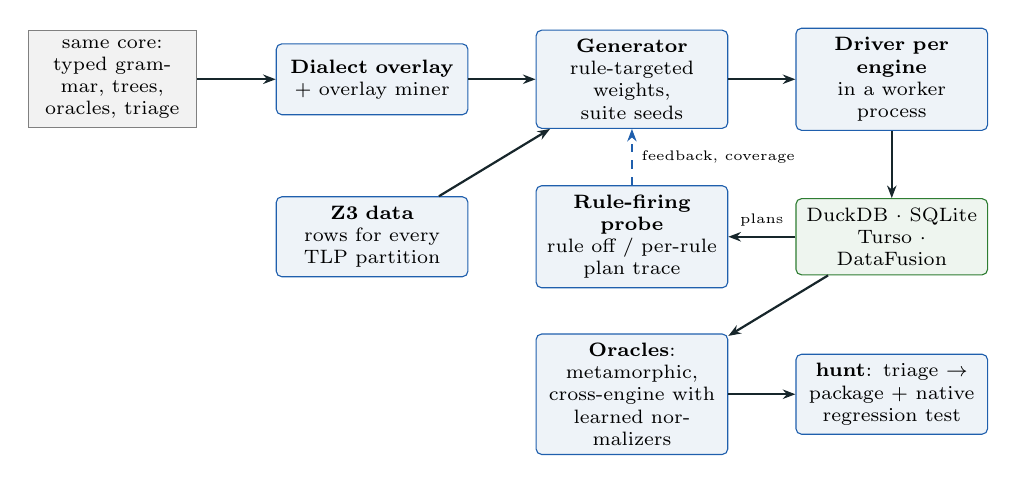
\begin{tikzpicture}
\node[io]  (core) at (0,0)     {same core: typed grammar, trees, oracles, triage};
\node[box] (ov)   at (3.3,0)   {\textbf{Dialect overlay}\\+ overlay miner};
\node[box] (gen)  at (6.6,0)   {\textbf{Generator}\\rule-targeted weights,\\suite seeds};
\node[box] (drv)  at (9.9,0)   {\textbf{Driver per engine}\\in a worker process};
\node[box] (z3)   at (3.3,-2)  {\textbf{Z3 data}\\rows for every\\TLP partition};
\node[box] (rule) at (6.6,-2)  {\textbf{Rule-firing probe}\\rule off / per-rule\\plan trace};
\node[orc] (eng)  at (9.9,-2)  {DuckDB $\cdot$ SQLite\\Turso $\cdot$ DataFusion};
\node[box] (orc)  at (6.6,-4)  {\textbf{Oracles}: metamorphic,\\cross-engine with\\learned normalizers};
\node[box] (hunt) at (9.9,-4)  {\textbf{hunt}: triage $\rightarrow$\\package + native\\regression test};
\draw[fl] (core)--(ov); \draw[fl] (ov)--(gen); \draw[fl] (gen)--(drv); \draw[fl] (drv)--(eng);
\draw[fl] (z3)--(gen);
\draw[fl] (eng)--node[above,font=\tiny]{plans}(rule);
\draw[bk] (rule)--node[right,font=\tiny]{feedback, coverage}(gen);
\draw[fl] (eng)--(orc); \draw[fl] (orc)--(hunt);
\end{tikzpicture}
}
\scriptsize
\begin{columns}[T]
\column{0.5\textwidth}
\begin{itemize}
  \item \textbf{Driver per engine} in a worker process (DuckDB, SQLite, Turso, DataFusion); same trees, oracles, triage.
  \item \textbf{Dialect overlays} on the same grammar + \textbf{overlay miner} (79--98\% valid).
  \item \textbf{Optimizer-rule firing} instead of code coverage: feedback, coverage, rule-targeted generation.
\end{itemize}
\column{0.5\textwidth}
\begin{itemize}
  \item \textbf{Z3 data synthesis}: rows for every TLP partition.
  \item \textbf{Learned normalizers}: cross-engine comparison (disagreements 28.7\% $\rightarrow$ 3.6\%).
  \item \textbf{Autonomous loop}: campaign $\rightarrow$ triage $\rightarrow$ package with a regression test in the engine's own format.
\end{itemize}
\end{columns}
\end{frame}
\note{VENU (45 s). We made the tool target-independent. Each engine gets a driver and a dialect
overlay on the same grammar; a miner drafts the overlay from failure rates. Instead of
PostgreSQL's planner settings we observe which optimizer rules fire, which works on any release
build. Z3 makes metamorphic checks non-vacuous, learned normalizers let us compare two engines, and
the hunt loop goes from campaign to a filing package on its own.}

\begin{frame}{Generalized fuzzer: three bugs in detail}
\scriptsize
\begin{columns}[T]
\column{0.32\textwidth}
\begin{block}{Turso}
\textbf{State}: \wa{filed with fix}\\[2pt]
\textbf{Type}: wrong result / spurious error.\\[2pt]
\textbf{What happened}: \texttt{percentile\_disc}/\texttt{percentile\_cont} read their arguments from consecutive registers, but an expression argument was compiled into a temporary register, so the aggregate read the wrong value.\\[2pt]
\textbf{How found}: Turso-vs-SQLite differential oracle; reduced to one aggregate call.\\[2pt]
\textbf{Fix}: arguments compiled into one register block. Issue \#11594, PR \#11595 (12{,}700 tests pass).
\end{block}
\column{0.32\textwidth}
\begin{block}{DuckDB}
\textbf{State}: \ok{approved by a maintainer}\\[2pt]
\textbf{Type}: internal error, regression in 2.0.0.\\[2pt]
\textbf{What happened}: for \texttt{min}/\texttt{max} over a nested value the binder copied the argument before checking whether a collation applies; an argument containing a subquery cannot be copied.\\[2pt]
\textbf{How found}: internal-error oracle on the nightly build.\\[2pt]
\textbf{Fix}: copy only when a collation applies. Issue \#28551, PR \#28552 (collation and subquery suites pass).
\end{block}
\column{0.32\textwidth}
\begin{block}{DataFusion}
\textbf{State}: \wa{filed with fix}\\[2pt]
\textbf{Type}: internal error in \texttt{UPDATE}/\texttt{DELETE}.\\[2pt]
\textbf{What happened}: common-subexpression elimination replaced a repeated expression by a column that exists only in the plan; DML then asked the table for that column.\\[2pt]
\textbf{How found}: internal-error oracle; re-check on \texttt{main} found the \texttt{WHERE} clause fails too.\\[2pt]
\textbf{Fix}: inline such columns before DML. Issue \#27235, PR \#27236 (all 546 test files pass).
\end{block}
\end{columns}
\smallskip
\scriptsize \textbf{Other bugs found}: a DataFusion internal error with subqueries in \texttt{VALUES} and a Turso panic with an aggregate in \texttt{IN (SELECT ...)} next to a window function (both with a fix ready); a Turso panic, a rejected Turso join and a DuckDB bind error, all three already fixed upstream when we re-checked on the newest code (\texttt{main}).
\end{frame}
\note{GOWTHAM (20 s) Turso: only the comparison with SQLite showed the wrong value; the aggregate
read its fraction from the wrong register. BHUVAN (20 s) DuckDB: the internal-error oracle; a
2.0.0 change made the binder copy an expression that cannot be copied. VENU (20 s) DataFusion: an
optimizer rule leaked a plan-only column into UPDATE and DELETE. All three pull requests carry a
regression test and pass the engine's full test suite.}

\begin{frame}{Results and conclusion}
\begin{columns}[T]
\column{0.24\textwidth}\centering{\Huge\textbf{9}}\\\scriptsize \pg bugs reported
\column{0.24\textwidth}\centering{\Huge\ok{7}}\\\scriptsize fixed upstream (5 our patches)
\column{0.24\textwidth}\centering{\Huge\textbf{3}}\\\scriptsize fixes filed to DuckDB, Turso, DataFusion
\column{0.24\textwidth}\centering{\Huge\textbf{36.7\%}}\\\scriptsize backend lines (random 22.2\%)
\end{columns}
\bigskip
\small
\begin{itemize}
  \item Evaluation: 5 trials $\times$ 1 h per arm; 93 candidates triaged; 23 re-injected real bugs as ground truth.
  \item Lesson: valid SQL is the easy part; \alert{oracle precision} decides how useful a fuzzer is.
  \item Team: Venu (tool, paper, generalized fuzzer) $\cdot$ Bhuvan (benchmark, bug hunts, four patches) $\cdot$ Gowtham (campaigns, LLM arm, two reports, one fix).
\end{itemize}
\end{frame}
\note{BHUVAN (30 s). Typed generation reaches far more backend code than random mutation, and the
oracles find bugs a crash fuzzer cannot see. Our main lesson: precision of the oracles is the
limit. Thank you.}

\begin{frame}[standout]
Thank you. Questions?\\[6pt]
\normalsize github.com/PASS-IITG/cs5187-term-project-blazing-bhuvi
\end{frame}

\end{document}
